\documentclass[14pt,xcolor=pdftex,dvipsnames,table]{beamer}\usepackage[]{graphicx}\usepackage[]{color}
%% maxwidth is the original width if it is less than linewidth
%% otherwise use linewidth (to make sure the graphics do not exceed the margin)
\makeatletter
\def\maxwidth{ %
  \ifdim\Gin@nat@width>\linewidth
    \linewidth
  \else
    \Gin@nat@width
  \fi
}
\makeatother

\definecolor{fgcolor}{rgb}{0.345, 0.345, 0.345}
\newcommand{\hlnum}[1]{\textcolor[rgb]{0.686,0.059,0.569}{#1}}%
\newcommand{\hlstr}[1]{\textcolor[rgb]{0.192,0.494,0.8}{#1}}%
\newcommand{\hlcom}[1]{\textcolor[rgb]{0.678,0.584,0.686}{\textit{#1}}}%
\newcommand{\hlopt}[1]{\textcolor[rgb]{0,0,0}{#1}}%
\newcommand{\hlstd}[1]{\textcolor[rgb]{0.345,0.345,0.345}{#1}}%
\newcommand{\hlkwa}[1]{\textcolor[rgb]{0.161,0.373,0.58}{\textbf{#1}}}%
\newcommand{\hlkwb}[1]{\textcolor[rgb]{0.69,0.353,0.396}{#1}}%
\newcommand{\hlkwc}[1]{\textcolor[rgb]{0.333,0.667,0.333}{#1}}%
\newcommand{\hlkwd}[1]{\textcolor[rgb]{0.737,0.353,0.396}{\textbf{#1}}}%

\usepackage{framed}
\makeatletter
\newenvironment{kframe}{%
 \def\at@end@of@kframe{}%
 \ifinner\ifhmode%
  \def\at@end@of@kframe{\end{minipage}}%
  \begin{minipage}{\columnwidth}%
 \fi\fi%
 \def\FrameCommand##1{\hskip\@totalleftmargin \hskip-\fboxsep
 \colorbox{shadecolor}{##1}\hskip-\fboxsep
     % There is no \\@totalrightmargin, so:
     \hskip-\linewidth \hskip-\@totalleftmargin \hskip\columnwidth}%
 \MakeFramed {\advance\hsize-\width
   \@totalleftmargin\z@ \linewidth\hsize
   \@setminipage}}%
 {\par\unskip\endMakeFramed%
 \at@end@of@kframe}
\makeatother

\definecolor{shadecolor}{rgb}{.97, .97, .97}
\definecolor{messagecolor}{rgb}{0, 0, 0}
\definecolor{warningcolor}{rgb}{1, 0, 1}
\definecolor{errorcolor}{rgb}{1, 0, 0}
\newenvironment{knitrout}{}{} % an empty environment to be redefined in TeX

\usepackage{alltt}

% Specify theme
\usetheme{Madrid}
% See deic.uab.es/~iblanes/beamer_gallery/index_by_theme.html for other themes
\usepackage{caption}
\usepackage{tikz}
\usepackage{multirow}
% Specify base color
\usecolortheme[named=OliveGreen]{structure}
% See http://goo.gl/p0Phn for other colors

% Specify other colors and options as required
\setbeamercolor{alerted text}{fg=Maroon}
\setbeamertemplate{items}[square]

% Title and author information
\title{Elasticity}
\author{Rob Hayward}
\IfFileExists{upquote.sty}{\usepackage{upquote}}{}
\begin{document}

\begin{frame}
\titlepage
\end{frame}


\section{Introduction}
\begin{frame}{Introduction}
Economics is all about relationships between variables.  We will look at three main types.  These all assess the change in demand.  Remember, demand will fall as the price increases.  Elasticity attempts to quantify that relationship.
\begin{itemize}[<+-| alert@+>]
\item Price-elasticity of demand
\item Income elasticity of demand
\item Cross-price elasticity of demand
\end{itemize}
\end{frame}

\begin{frame}{Determinants of elasticity}
Five factors determine elasticity.
\begin{itemize}[<+-| alert@+>]
\item Availability of substitutes
\item Necessities vs luxuries
\item Definition of the market
\item Proportion of income devoted to the product
\item Time horizon
\end{itemize}
\end{frame}

\begin{frame}{Price elasticity of demand}
Elasticity is the percentage change in quantity demanded relative to the change in price.
\begin{align*}
ped &= \frac{\text{percentage change in quantity demanded}}{\text{percentage change in price}}\\
      & = \frac{\%\Delta Q_d}{\%\Delta P}
\end{align*}
\end{frame}

\begin{frame}{Example (ped)}
\begin{itemize}[<+-| alert@+>]
\item The price of coffee increases by 4\%
\item The demand for coffee falls by 2\%
\end{itemize}
\pause
\begin{align*}
ped &= \frac{-2}{4}\\
&= -0.5
\end{align*}
\end{frame}

\begin{frame}{Price elasticity of demand}
\begin{itemize}[<+-| alert@+>]
\item The price elasticity of demand is negative
\item It can range from zero to minus infinity
\item Between zero and minus one, usually say it is inelastic
\item Above one, it is elastic
\item Usually speak in terms of relative elasticity
\end{itemize}
\end{frame}

\begin{frame}{Measuring elasticity}
There are two ways of measuring elasticity 
\begin{itemize}[<+-| alert@+>]
\item Mid-point or arc elasticity of demand
\item Point elasticity of demand
\end{itemize}
\end{frame}

\begin{frame}{Example}
If there are two points
\begin{itemize}[<+-| alert@+>]
\item Point A:  P = 4, Q = 120
\item Point B: P = 6, Q = 80
\end{itemize}
\pause
\begin{align*}
ped(A - B) &= \frac{-33}{+50} = 0.66\\
ped(B - A) & = \frac{+50}{-33} = 1.5
\end{align*}
\end{frame}

\begin{frame}{Solution}
Calculate the percentage from the mid-point rather than the starting point. 
\begin{align*}
\% \Delta P =& \frac{2}{5} = 0.4\\
\% \Delta Q =& \frac{40}{100} = 0.4\\
ped = &\frac{0.4}{0.4} = 1
\end{align*}
\end{frame}

\begin{frame}{Solution}
Calculation 
\begin{equation*}
ped = \frac{(Q_2 - Q_1)/[(Q_2 - Q_1)/2]}{(P_2 - P_1)/[(P_2 - P_1)/2]}
\end{equation*}
\end{frame}

\begin{frame}{Point Elasticity of Demand}
Elasticity is 
\begin{align*}
ped =& \frac{\%\Delta Q_d}{\% \Delta P}\\
= & \frac{\Delta Q_d}{Q_d}/\frac{\Delta P}{P}\\
= & \frac{\Delta Q}{\Delta P} \times  \frac{P}{Q_d}
\end{align*}
Or (reciprical) of the slope multiplied by point
\end{frame}

\begin{frame}{Point elasticity calculation}
\begin{tikzpicture}[scale = 2]
%\usetiktzlibrary{calc}
%\draw[very thin, color = gray](0, 0) grid (5, 3);
\draw [<->, thick] (0, 3) node (yaxis) [above] {$P$} 
  |- (5, 0) node (xaxis) [right] {$Q_d$};
\node at (1, 0) [below] {$1$};
\node at (2, 0) [below] {$2$};
\node at (3, 0) [below] {$3$};
\node at (4, 0) [below] {$4$};
\node at (0, 1) [left] {$1$};
\node at (0, 2) [left] {$2$};
\node at (0, 3) [left] {$3$};
\draw[domain = 0.1:3.9, color = blue] plot(\x, {2 - 0.5*\x});
\node at (3, 3) {$P = 2 - 0.5Q_d$};
\node at (3, 2) {$Slope = -0.5$};
\pause
\fill (2, 1) circle (2pt);
\end{tikzpicture}
\end{frame}

\begin{frame}{Calculation of point elasticity at $(2, 1)$}
The equation for point elasticity is 
\begin{equation*}
ped =  \frac{\Delta Q_d}{\Delta P} \times  \frac{P}{Q_d}
\end{equation*}
Therefore, 
\begin{align*}
ped = & \frac{1}{0.5} \times  \frac{1}{2}\\
=& \frac{2}{2} = 1
\end{align*}
\end{frame}

\begin{frame}{Elasticities: Relatively elastic}
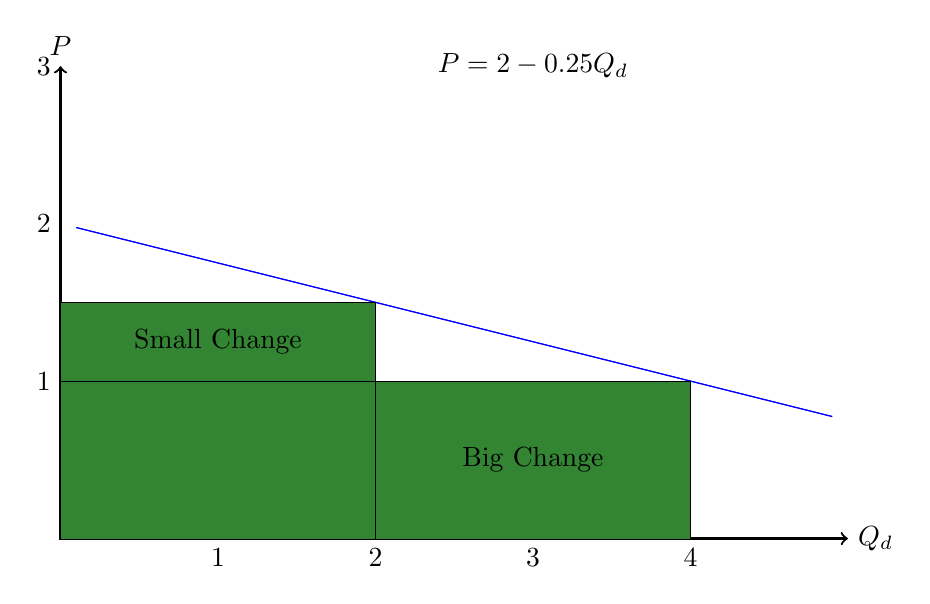
\begin{tikzpicture}[scale = 2]
%\usetiktzlibrary{calc}
%\draw[very thin, color = gray](0, 0) grid (5, 3);
\draw [<->, thick] (0, 3) node (yaxis) [above] {$P$} 
  |- (5, 0) node (xaxis) [right] {$Q_d$};
\node at (1, 0) [below] {$1$};
\node at (2, 0) [below] {$2$};
\node at (3, 0) [below] {$3$};
\node at (4, 0) [below] {$4$};
\node at (0, 1) [left] {$1$};
\node at (0, 2) [left] {$2$};
\node at (0, 3) [left] {$3$};
\draw[domain = 0.1:4.9, color = blue] plot(\x, {2 - 0.25*\x});
\def\demand{\x, {2 - 0.25*\x}};
\fill [fill = black!60!green!80] (4, 0) -- (0, 0) -- (0, 1) -- (4, 1) -- cycle;
\fill [fill = black!60!green!80] (2, 0) -- (0, 0) --(0, 1.5) -- (2, 1.5) -- cycle;
\draw[domain = 0.1:4.9, color = blue] plot(\x, {2 - 0.25*\x});
\draw  (2,0) -- (2, 1.5);
\draw  (4,0) -- (4, 1);
\draw  (0,1) -- (4, 1);
\draw (0, 1.5) -- (2, 1.5);
\node at (3, 3) {$P = 2 - 0.25Q_d$};
%\node at (3, 2) {Relatively Elastic};
\node at (3, 0.5) {Big Change};
\node at (1, 1.25) {Small Change};
%\fill (2, 1) circle (2pt);
\end{tikzpicture}
\end{frame}

\begin{frame}{Elasticities: relatively in-elastic}
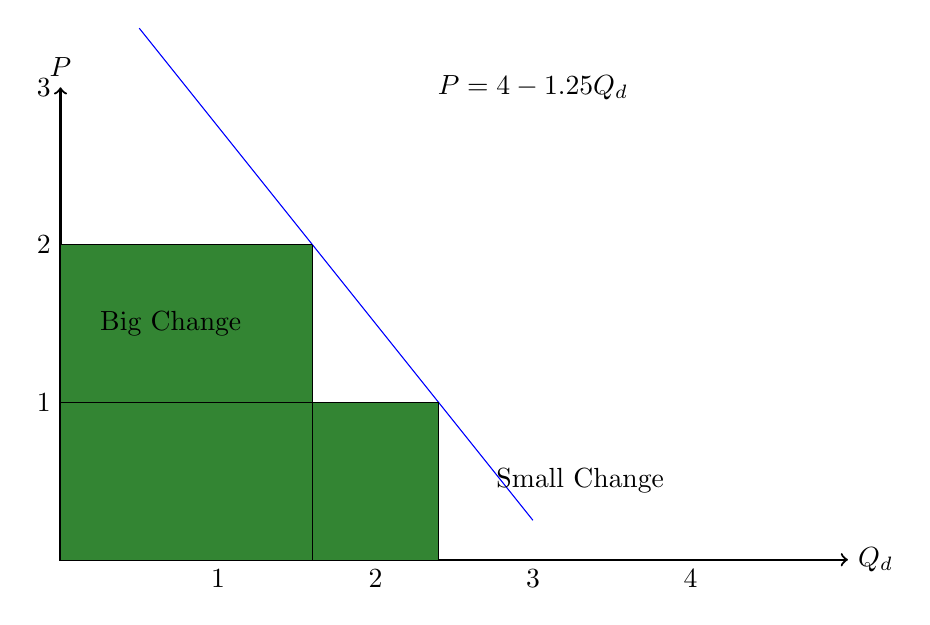
\begin{tikzpicture}[scale = 2]
%\usetiktzlibrary{calc}
%\draw[very thin, color = gray](0, 0) grid (5, 3);
\draw [<->, thick] (0, 3) node (yaxis) [above] {$P$} 
  |- (5, 0) node (xaxis) [right] {$Q_d$};
\node at (1, 0) [below] {$1$};
\node at (2, 0) [below] {$2$};
\node at (3, 0) [below] {$3$};
\node at (4, 0) [below] {$4$};
\node at (0, 1) [left] {$1$};
\node at (0, 2) [left] {$2$};
\node at (0, 3) [left] {$3$};
\draw[domain = 0.5:3, color = blue] plot(\x, {4 - 1.25*\x});
\def\demand{\x, {4 - 1.25 * \x}};
\fill [fill = black!60!green!80] (2.4,0) -- (0, 0) -- (0, 1) -- (2.4, 1) -- cycle;
\fill [fill = black!60!green!80] (1.6, 0) -- (0, 0) -- (0, 2) -- (1.6, 2) -- cycle;
%\draw[domain = 0.1:4.9, color = blue] plot(\x, {4 - 1.25*\x});
\draw  (2.4,0) -- (2.4, 1);
\draw  (1.6, 0) -- (1.6, 2);
\draw  (0,1) -- (2.4, 1);
\draw (0, 2) -- (1.6, 2);
\node at (3, 3) {$P = 4 - 1.25Q_d$};
%\node at (3, 2) {Relatively In-elastic};
\node at (0.7, 1.5) {Big Change};
\node at (3.3, 0.5) {Small Change};
%\fill (2, 1) circle (2pt);
\end{tikzpicture}
\end{frame}

\begin{frame}{Elasticity changes through the demand curve}
\begin{tikzpicture}[scale = 2]
%\usetiktzlibrary{calc}
%\draw[very thin, color = gray](0, 0) grid (5, 3);
\draw [<->, thick] (0, 3) node (yaxis) [above] {$P$} 
  |- (5, 0) node (xaxis) [right] {$Q_d$};
\node at (1, 0) [below] {$1$};
\node at (2, 0) [below] {$2$};
\node at (3, 0) [below] {$3$};
\node at (4, 0) [below] {$4$};
\node at (0, 1) [left] {$1$};
\node at (0, 2) [left] {$2$};
\node at (0, 3) [left] {$3$};
\draw[domain = 0.1:3.9, color = blue] plot(\x, {2 - 0.5*\x});
\node at (1, 1.8) {Elastic};
\node at (3.7, 0.5) {Inelastic};
\fill (2, 1) circle (2pt);
\node at (2, 1) [right] {Unit Elasticity};
\end{tikzpicture}
\end{frame}

\begin{frame}{Income elasticity of demand}
Income elasticity of demand is the percentage change in quantity demanded relative to the change in income.
\begin{align*}
ied &= \frac{\text{percentage change in quantity demanded}}{\text{percentage change in income}}\\
      & = \frac{\%\Delta Q_d}{\%\Delta Y}
\end{align*}
Normal good have a positive relationship, luxury is above 1 and \emph{inferior} is a negative relationship.
\end{frame}

\begin{frame}{Cross-price elasticity of demand}
Elasticity is the percentage change in quantity demanded relative to the change in price.
\begin{align*}
xped &= \frac{\text{percentage change in quantity demanded good i}}{\text{percentage change in price of good j}}\\
      & = \frac{\%\Delta Q_{d, i}}{\%\Delta P_j}
\end{align*}
Positive relationship for substitutes and negative for compliments. 
\end{frame}

\begin{frame}{Importance of elasticity}
Why care about eleasticity?
\begin{itemize}[<+-| alert@+>]
\item Monopolist should raise prices while demand is inelastic and drop them when demand is elastic
\item Luxury or normal or inefrior goods
\item Importance of competitors' actions (oligopoly and monopolistic competition)
\item Price discrimination
\end{itemize}
\end{frame}




\begin{frame}{Price Discrimination}
Charging different prices for the same product
\begin{itemize}[<+-| alert@+>]
\item There must be some element of market power
\item \emph{perfect price discrimination will change a unique price to each buyer}
\item Related to market segmentation
\item Need to identify the elasticity of demanad for groups of customers
\item Need to make sure that buyers cannot swap between markets
\end{itemize}
\end{frame}

\begin{frame}{Price Discrimination}
\includegraphics<1>[width=12cm, height=9cm]{"../Figures/train"}
\end{frame}



\end{document}
